\chapter{MIP Approach}
\label{chapter-mip}

TODO rigorously define MIP - optimization problem similar to LP, however some of the variables integral or boolean

TODO FIDAX is cool, but their heuristic might not be the best. It is a IS problem, let's try a multi-purpose solver. Use GLPK. \nomenclature{GLPK}{GNU Linear Programming Kit}

\section{Finding ID sets with GLPK}

TODO how GLPK works (branch \& bound), how to construct a problem, how output looks, how to interpret it, limit time-> limit quality, ...

TODO define \textit{name(AM)}

\begin{verbatim}
<x>
  <y a="1" b="2"/>
  <y a="3" c="4"/>
  <y/>
  <z a="1"/>
</x>
\end{verbatim}

TODO equations for the MIP formulation

\begin{scriptsize}
\begin{verbatim}
set AMs;
param Weight {i in AMs};
var x {i in AMs} binary;
maximize z: sum {i in AMs} x[i] * Weight[i];
s.t. c1: x['y-b'] + x['y-c'] <= 1;
s.t. c2: x['y-a'] + x['y-c'] <= 1;
s.t. c3: x['y-a'] + x['y-b'] <= 1;
s.t. c4: x['y-a'] + x['z-a'] <= 1;
data;
set AMs :=
y-c
y-b
y-a
z-a;
param Weight :=
y-c 0.2
y-b 0.2
y-a 0.6
z-a 0.4;
end;
\end{verbatim}
\end{scriptsize}

 -> wow, GLPK works. However, it takes too long to get to optimum (link experiments), so let's try other heuristics.

\section{Heuristics}

TODO what is heuristics (link wise books), what is metaheuristics (we will be using them)

TODO mention things like Taboo search and Genetic Algorithms (we can emulate them with Crossover/Mutation) (we won't be using them)

TODO we will be working with heuristics striving to do the following: input is a list of AMs, they have their weight, we try to find a non-conflicting subset which maximizes the weight

TODO we will be using a pool - what is a pool

\begin{figure}
  \caption{Metaheuristic schema}
  \label{image-metaheuristic}
  \centering
    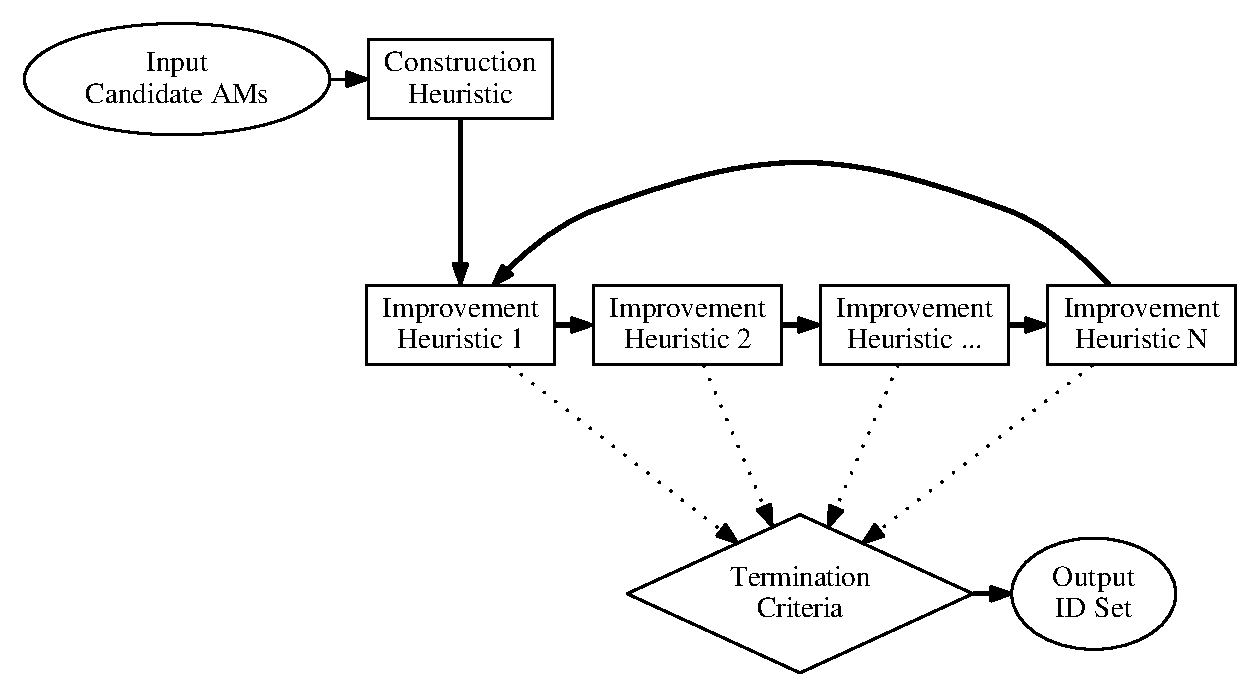
\includegraphics[width=\textwidth]{images/metaheuristic}
\end{figure}

\subsection{Constructions Heuristics}
% TODO can I format things in nomenclature?
\nomenclature{CH}{Construction Heuristic} %TODO decide on how to format CH/IH

TODO construction heuristics are heus that provide us with at least some solution.

\subsubsection{\heu{FIDAX}}

It should be obvious by now that the algorithm described in \cite{fidax} (we shall call it \heu{FIDAX} from now on) can trivially be used as a construction heuristic that will give us one feasible solution.

The pseudocode of this CH (taken from the original article with trivial modifications without changing the logic) is in Listing \ref{listing-ch-fidax}.

\begin{algorithm}
\caption{\heu{FIDAX} CH}
\label{listing-ch-fidax}
\begin{algorithmic}
\REQUIRE $C$ list of candidate AMs
\ENSURE a feasible solution
\STATE $C' \gets C$ sorted by decreasing size
\STATE Compute the weight $w(m)$ of each $m$ in $C$
\FORALL{$t$ in $\Sigma^E$}
  \STATE Let $m$ be a \textbf{highest-weight} mapping of type $t$ in $C'$
  \STATE Remove from $C'$ all mappings of type $t$ except $m$
\ENDFOR
\FORALL{$m$ in $C'$}
  \STATE $S \gets$ all mappings in $C$ whose images intersect $\iota(m)$
  \IF{$w(m) > \sum_{p \in S} w(p)$}
    \STATE remove all $p \in S$ from $C'$
  \ELSE
    \STATE remove $m$ from $C'$
  \ENDIF
\ENDFOR
\RETURN $C'$
\end{algorithmic}
\end{algorithm}

\subsubsection{\heu{Random}}
\label{heu-ch-random}

One of the most natural heuristics when dealing with the IS problem can be described as follows: select from candidate AMs at random, if possible (addition would not violate the ID set condition) add them to the solution. This is obviously a hungry heuristic. %TODO have I defined ID set condition yet??

The advantages of this trivial heuristic are simplicity, speed and ease with which it can create a pool of variable solutions, almost for free. As we will see later in the experiments (Section \ref{section-experiments-random-fuzzy-fidax}), it performs surprisingly well.

See the Listing \ref{listing-ch-random} for its pseudocode.

\begin{algorithm}
\caption{\heu{Random} CH}
\label{listing-ch-random}
\begin{algorithmic}
\REQUIRE $N$ required size of pool
\REQUIRE $C$ list of candidate AMs
\ENSURE pool of $N$ feasible solutions
\STATE $r \gets $ empty pool
\FOR{$i = 1 \to N$}
  \STATE \COMMENT{create 1 solution}
  \STATE $s \gets $ empty solution
  \WHILE{$s$ is a feasible ID set}
    \STATE $a \gets $ pick at random from $C \backslash S$
    \STATE $s \gets s \cup a$
  \ENDWHILE
  \STATE $r \gets r \cup s$
\ENDFOR
\RETURN $r$
\end{algorithmic}
\end{algorithm}

\subsubsection{\heu{Fuzzy}}
\label{heu-ch-fuzzy}

\heu{Fuzzy} is an improvement over the \heu{Random} CH: it picks the next AM to try to add based on \textit{weighted} instead of uniform random. The weight used here is the usual weight of an AM as defined in TODO. Because of the randomness involved in the choice, we can again easily create a pool of solutions this way.

Again, this is a hungry heuristic, the Listing \ref{listing-ch-fuzzy} contains its pseudocode.

% TODO od I need to specify which are my own idea? I guess so, I should link any heu that is not mine. But do I need to stress that for example Fuzzy is mine?

\begin{algorithm}
\caption{\heu{Fuzzy} CH}
\label{listing-ch-fuzzy}
\begin{algorithmic}
\REQUIRE $N$ required size of pool
\REQUIRE $C$ list of candidate AMs
\ENSURE pool of $N$ feasible solutions
\STATE $r \gets $ empty pool
\FOR{$i = 1 \to N$}
  \STATE \COMMENT{create 1 solution}
  \STATE $s \gets $ empty solution
  \STATE $C' \gets C$

  \WHILE{$C' $ not empty}
    \STATE $a \gets $ pick at weighted random from $C'$
    \IF{$s \cup a$ is a feasible ID set}
      \STATE $s \gets s \cup a$
      \STATE $C' \gets C' \backslash a$
    \ENDIF
    \FORALL{$c \in C'$}
      \IF{$s \cup c $ is \textbf{not} a feasible ID set}
        \STATE \COMMENT {if $c$ cannot be possibly added anymore}
        \STATE $C' \gets C' \backslash c$
      \ENDIF
    \ENDFOR
  \ENDWHILE

  \STATE $r \gets r + s$
\ENDFOR
\RETURN $r$
\end{algorithmic}
\end{algorithm}

\subsubsection{\heu{Incremental}}

This trivial heuristics sorts all candidate AMs by their decreasing weights (TODO link definition of weight) and then tries to iteratively add them to solution, if possible. This way it can create only one solution, and again, this is a hungry heuristic.

See listing \ref{listing-ch-incremental}.

\begin{algorithm}
\caption{\heu{Incremental} CH}
\label{listing-ch-incremental}
\begin{algorithmic}
\REQUIRE $C$ list of candidate AMs
\ENSURE a feasible solution
\STATE $C' \gets $ sort $C$ by decreasing weight
\STATE $s \gets $ empty solution
\FORALL{$c \in C'$}
  \IF{$s \cup c$ is a feasible ID set}
    \STATE $s \gets s + c$
  \ENDIF
\ENDFOR
\RETURN $s$
\end{algorithmic}
\end{algorithm}

\subsubsection{\heu{Removal}}

This is basically a reversal of the idea from the \heu{Incremental} heuristic - start with a solution containing all the candidate AMs. This probably does not satisfy the ID set condition. Therefore, order them by increasing size and start removing them from the solution, until it satisfies the ID set condition. Again, this is a hungry heuristic returning only one solution.

See listing \ref{listing-ch-removal}.

\begin{algorithm}
\caption{\heu{Removal} CH}
\label{listing-ch-removal}
\begin{algorithmic}
\REQUIRE $C$ list of candidate AMs
\ENSURE a feasible solution
\STATE $C' \gets $ sort $C$ by increasing weight
\STATE $s \gets C'$
\FORALL{$c \in s$}
  \IF{$s$ is a feasible ID set}
    \RETURN $s$
  \ENDIF
  \STATE $s \gets s \backslash c$
\ENDFOR
\end{algorithmic}
\end{algorithm}

\subsubsection{Truncated Branch \& Bound}

This CH will be called \heu{Glpk} from now on, for it is basically a time-constrained run of GLPK.

TODO if we limit GLPK's runtime, we get this

TODO we shuffle AMs - we get different runs - pool is possible

\subsection{Improvement Heuristics}
\label{section-mip-ihs}

\nomenclature{IH}{Improvement Heuristic}

TODO what they are, that they need a pool sometimes, their input and output is a pool, ...

TODO mention intensification, diversification

TODO mention that combination of \heu{Crossover}, \heu{Mutation} and \heu{RemoveWorst} is a sort of genetic algorithm

\subsubsection{\heu{Identity}}

This ultimately trivial improvement heuristics does nothing. It simply returns the feasible pool unchanged. For the sake of completeness, see its listing \ref{listing-ih-identity}.

\begin{algorithm}
\caption{\heu{Identity} IH}
\label{listing-ih-identity}
\begin{algorithmic}
\REQUIRE $FP$ pool of feasible solutions
\ENSURE the same pool of feasible solutions
\RETURN $FP$
\end{algorithmic}
\end{algorithm}

\subsubsection{\heu{Remove Worst}}

This trivial IH tries to improve the solution pool by removing the worst solution (i.e. the one with the lowest quality). This might be interesting in cooperation with other improvement heuristics that increase the solution pool size, to keep it from growing by pruning inferior solutions.

See listing \ref{listing-ih-removeworst}.

\begin{algorithm}
\caption{\heu{Remove Worst} IH}
\label{listing-ih-removeworst}
\begin{algorithmic}
\REQUIRE $FP$ pool of feasible solutions
\ENSURE pool of feasible solutions
\STATE $s_{min} \gets $ solution with the lowest weight $\in FP$
\RETURN $FP \backslash s_{min}$
\end{algorithmic}
\end{algorithm}

\subsubsection{\heu{Random Remove}}

This is again a rather trivial IH, something which is usually referred to as a \textit{perturbation} function. % TODO link the notion
By removing a random subset of specified size from each solution in the pool, it provides variability needed to escape from local optima. % TODO make sure we have talked about local optima before

The number of AMs to remove from each solution is specified as ratio (from the interval $(0, 1)$) of the solution size. % TODO have we defined what a solution size is?
For example, \heu{Random Remove} with $ratio = 0.1$ would remove 1 random AM from a solution containing 10 AMs and 2 from a solution containing 17 AMs (due to rounding).

This heuristic returns a pool of solutions of the same size as it got on its input.

See listing \ref{listing-ih-randomremove}.

\begin{algorithm}
\caption{\heu{Random Remove} IH}
\label{listing-ih-randomremove}
\begin{algorithmic}
\REQUIRE $FP$ pool of feasible solutions
\REQUIRE $k \in (0,1)$ ratio of AMs to remove from each $s \in FP$
\ENSURE pool of feasible solutions
\FORALL{$s \in FP$}
  \STATE $K \gets k * |s|$
  \STATE remove $K$ random AMs from $s$
\ENDFOR
\RETURN $FP$
\end{algorithmic}
\end{algorithm}

\subsubsection{\heu{Hungry}}

This simple improvement heuristic assumes that the solutions in the pool are not ``complete", i.e. there are AMs that could be added to them without violating the ID set condition.

\heu{Hungry} tries to improve each solution in the feasible pool in the following way. It orders all candidate AMs not present in the solution by decreasing weight. Afterwards, it iteratively tries to extend the solution with these AMs, taking care not to violate the ID set condition. The resulting solution (whether any AMs were added or not) is then returned to the pool. Listing \ref{listing-ih-hungry} captures this process.

\begin{algorithm}
\caption{\heu{Hungry} IH}
\label{listing-ih-hungry}
\begin{algorithmic}
\REQUIRE $FP$ pool of feasible solutions
\REQUIRE $C$ list of candidate AMs
\ENSURE pool of feasible solutions
\FORALL{$s \in FP$}
  \STATE \COMMENT {improve a single solution}
  \STATE $C' \gets C \backslash s$
  \STATE $C' \gets C'$ sorted by decreasing weight
  \FORALL{$c \in C'$}
    \IF{$s \cup c$ is a feasible ID set}
      \STATE $s \gets s \cup c$
    \ENDIF
  \ENDFOR
\ENDFOR
\RETURN $FP$
\end{algorithmic}
\end{algorithm}

\subsubsection{\heu{Mutation}}

TODO explain how this works and link wise books

TODO explain how this translates to GLPK input

For every AM $AM_F$ fixed to appear in the solution a following constraint is added to GLPK input:
\[s.t. f_{index}: x['name(AM_F)'] = 1;\]
$index$ is a unique integer to number all the constraints.

Additionaly, every other mapping $AM_i$ colliding with $AM_F$ ($\iff \iota(AM_F) \cap \iota(AM_i) \neq \emptyset$) will cause the following constraint to be added:
\[s.t. f_{index}: x['name(AM_i)'] = 0;\]
And the original constraint in form:
\[s.t. c_{index}: x['name(AM_F)'] + x['name(AM_i)'] <= 1;\]
will not be included.

See listing \ref{listing-ih-mutation}.

\begin{algorithm}
\caption{\heu{Mutation} IH}
\label{listing-ih-mutation}
\begin{algorithmic}
\REQUIRE $FP$ pool of feasible solutions
\REQUIRE $k$ ratio of AMs to fix
\ENSURE pool of feasible solutions
\STATE $incumbent \gets $ best solution in $FP$ \COMMENT {best = highest weight}
\STATE $K \gets k * |incumbent|$
\STATE fix $K$ random AMs from $incumbent$ in GLPK problem formulation
\STATE $improved \gets $ run GLPK
\RETURN $FP \cup improved$
\end{algorithmic}
\end{algorithm}

\subsubsection{\heu{Crossover}}

TODO explain how this works and link wise books

TODO explain how this translates to GLPK input - it's again simple fixing to 1, but we get the list of AMs in a different manner.

See listing \ref{listing-ih-crossover}.

\begin{algorithm}
\caption{\heu{Crossover} IH}
\label{listing-ih-crossover}
\begin{algorithmic}
\REQUIRE $FP$ pool of feasible solutions
\REQUIRE $k$ ratio of solutions to look for commonalities in
\ENSURE pool of feasible solutions
\STATE $K \gets k * |FP|$
\STATE $FP' \gets K$ random solutions $\in FP$
\STATE $am \gets$ AMs found in all solutions $\in FP'$
\STATE fix $am$ in GLPK problem formulation
\STATE $improved \gets $ run GLPK
\RETURN $FP \cup improved$
\end{algorithmic}
\end{algorithm}

\subsubsection{\heu{Local Branching}}

TODO explain how this works and link wise books

TODO explain how this translates to GLPK input

A new constrain describing the maximal allowed distance from the incumbent solution is added to GLPK input.

\[s.t. LB: sum\{i\ in\ INCUMBENT\} (1 - x[i]) + sum\{i\ in\ REMAINING\} x[i] \leq k;\]

Where $INCUMBENT$ is a set of names of AMs in the incumbent solution, $REMAINING$ is a set of all the AMs not included in the incumbent solution and $k$ is the requested maximal distance.

See listing \ref{listing-ih-localbranching}.

\begin{algorithm}
\caption{\heu{Local Branching} IH}
\label{listing-ih-localbranching}
\begin{algorithmic}
\REQUIRE $FP$ pool of feasible solutions
\REQUIRE $k$ ratio of total AM count to bound the Hamming distance to
\ENSURE pool of feasible solutions
\STATE $K \gets k * |$total AM count$|$
\STATE $incumbent \gets $ best solution in $FP$ \COMMENT {best = highest weight}
\STATE add max Hamming distance requirement to GLPK problem formulation
\STATE $improved \gets $ run GLPK
\RETURN $FP \cup improved$
\end{algorithmic}
\end{algorithm}

\section{IDREF}

Once an ID set is found, regardless of how exactly, it is easy to find the IDREF set, i.e. the attribute mappings that can be declared as IDREF. % TODO link FIDAX, they did it first.

First of all, from the set of all the attribute mappings in the model remove all the AMs contained in the ID set. This is because the specification % TODO link to the specific anchor in the page
does not allow an attribute to be ID and IDREF (IDREFS) at the same time. Let us denominate these mappings as \textit{IDREF candidates} (obviously different from \textit{candidate AMs}). % TODO link candidate AMs

Second, find the image of the ID set as the union of images of all the AMs in this ID set.

\[\iota(ID) = \bigcup_{am \in ID} \iota(am)\]

Now the IDREF set contains all the AMs whose images are a subset of the ID set image.

\[\iota(c) \subset \iota(ID) \Rightarrow c \in IDREF\]

This can be easily determined in a loop over the list of candidates. The process is captured in Listing \ref{listing-idref}.

\begin{algorithm}
\caption{IDREF Search}
\label{listing-idref}
\begin{algorithmic}
\REQUIRE $AMs$ list of all AMs
\REQUIRE $ID$ ID set as a list of AMs
\ENSURE $IDREF$ set as a list of AMs
\STATE $IDREF \gets \emptyset$
\STATE $candidates \gets AMs \backslash ID$
\STATE $\iota(ID) \gets \bigcup_{am \in ID} \iota(am)$
\FORALL{$c \in candidates$}
  \IF{$\iota(c) \subset \iota(ID)$}
    \STATE $IDREF \gets IDREF \cup c$
  \ENDIF
\ENDFOR
\RETURN $IDREF$
\end{algorithmic}
\end{algorithm}
